\section{Why Is Intervention Needed Along the Student's Rollout?}
\label{sec:motivation}

\begin{figure}[!ht]
\centering
\captionsetup[subfigure]{font=scriptsize,skip=2pt}
\begin{subfigure}[t]{0.24\linewidth}
  \centering
  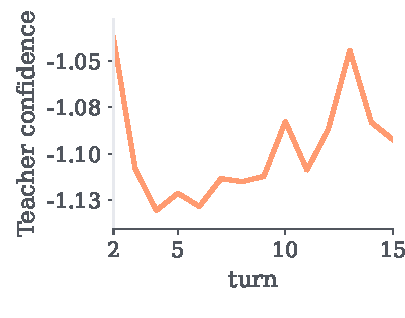
\includegraphics[width=\linewidth]{figures/fig_motivation_alfworld_confidence_depth.pdf}
  \caption{Student rollout}
\end{subfigure}\hfill
\begin{subfigure}[t]{0.24\linewidth}
  \centering
  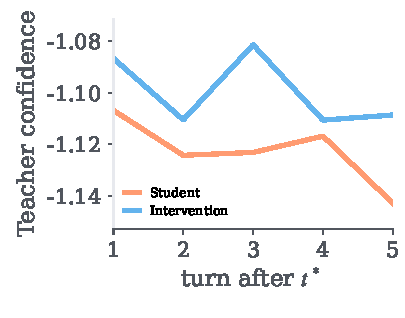
\includegraphics[width=\linewidth]{figures/fig_motivation_alfworld_confidence_recovery.pdf}
  \caption{After intervention}
\end{subfigure}\hfill
\begin{subfigure}[t]{0.24\linewidth}
  \centering
  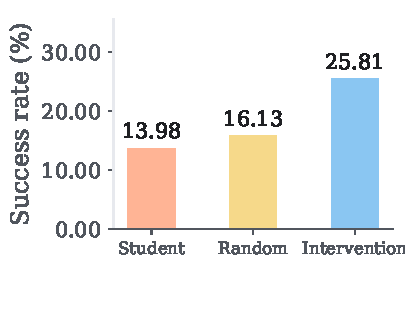
\includegraphics[width=\linewidth]{figures/fig_motivation_alfworld_performance.pdf}
  \caption{Intervention benefit}
\end{subfigure}\hfill
\begin{subfigure}[t]{0.24\linewidth}
  \centering
  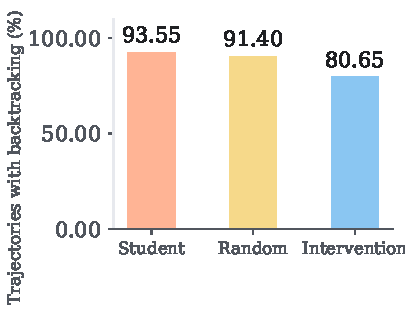
\includegraphics[width=\linewidth]{figures/fig_motivation_alfworld_state_return.pdf}
  \caption{Backtracking behavior}
\end{subfigure}

\caption{\textbf{One teacher intervention at a low-confidence step improves rollout quality.} (a) Teacher confidence fluctuates across turns of student-only rollouts. (b) Replacing one low-confidence action with a teacher action raises teacher confidence on subsequent actions generated by the student. (c)(d) This intervention increases task success and reduces backtracking compared with both student-only rollouts and random intervention. These results support using teacher uncertainty to select steps where a correction improves the rest of the rollout.}
\label{fig:motivation}
\end{figure}


 A poor student action can lead to further mistakes, affecting both task
  completion and the trajectory used for distillation. Standard OPD provides
  teacher supervision along this trajectory, but does not prevent the action
  from being executed. Correcting the action before execution can instead
  allow the student to continue from a better state and learn from the
  resulting trajectory. We therefore study whether teacher uncertainty
  identifies useful intervention points and whether a single teacher
  correction improves the student's subsequent rollout and task performance.

\noindent{\textbf{Experimental Setup.}}
We conduct a controlled study on ALFWorld \citep{shridhar2021alfworld}, keeping both models fixed. We use teacher confidence on student-generated actions to identify high-uncertainty steps. On the same tasks, we compare student-only rollouts, intervention at a low-confidence step, and intervention at a random step. Both intervention conditions replace exactly one student action with a teacher action, then return control to the student under the same turn limit. Appendix~\ref{app:motivation_details} provides the full protocol.

\noindent{\textbf{Observation 1: uncertainty varies across decision steps.}}
Teacher confidence falls and recovers along student rollouts (Fig.~\ref{fig:motivation}(a)), showing that the teacher's support for student-generated actions changes within an interaction. Low-confidence actions are weakly supported by the teacher and provide candidates for correction. In a multi-turn environment, executing such an action also determines the observations and decisions that follow, so its consequences can extend beyond the current turn. This motivates evaluating the student's proposed action in its current interaction history to decide when intervention may be useful.

\noindent{\textbf{Observation 2: one correction improves subsequent student behavior.}}
After intervention, the teacher assigns higher confidence to subsequent student-generated actions (Fig.~\ref{fig:motivation}(b)). The teacher acts only once, and the student resumes without any parameter update: the benefit extends to actions the student generates on its own after the correction. Task success also rises from approximately $14\%$ to $26\%$, compared with $16\%$ for random intervention (Fig.~\ref{fig:motivation}(c)). The two intervention conditions use the same amount of teacher assistance, yet selecting a low-confidence step produces a larger gain. These results show that both the action correction and its timing matter for the subsequent rollout.

\noindent{\textbf{Observation 3: intervention helps correct student errors.}}
Student errors can alter subsequent interaction and lead to behavior that fails to advance the task. We examine this effect in ALFWorld using returns to previously visited states as a task-specific behavioral indicator. Fig.~\ref{fig:motivation}(d) shows that low-confidence intervention reduces the fraction of trajectories that leave a state and later return to it, relative to both student-only rollouts and random intervention. Together with higher task success, this change suggests that a teacher correction can help the student recover from mistakes and make progress toward completing the task. A well-placed teacher correction can thus improve trajectory quality by changing how the student continues to act.

\noindent{\textbf{Takeaway.}}
Teacher correction at a high-uncertainty step improves subsequent student behavior and task success. Its advantage over random intervention shows that correction timing matters, motivating teacher uncertainty as a signal for deciding when to intervene.
